\documentclass[twoside]{book}

% Packages required by doxygen
\usepackage{fixltx2e}
\usepackage{calc}
\usepackage{doxygen}
\usepackage[export]{adjustbox} % also loads graphicx
\usepackage{graphicx}
\usepackage[utf8]{inputenc}
\usepackage{makeidx}
\usepackage{multicol}
\usepackage{multirow}
\PassOptionsToPackage{warn}{textcomp}
\usepackage{textcomp}
\usepackage[nointegrals]{wasysym}
\usepackage[table]{xcolor}

% Font selection
\usepackage[T1]{fontenc}
\usepackage[scaled=.90]{helvet}
\usepackage{courier}
\usepackage{amssymb}
\usepackage{sectsty}
\renewcommand{\familydefault}{\sfdefault}
\allsectionsfont{%
  \fontseries{bc}\selectfont%
  \color{darkgray}%
}
\renewcommand{\DoxyLabelFont}{%
  \fontseries{bc}\selectfont%
  \color{darkgray}%
}
\newcommand{\+}{\discretionary{\mbox{\scriptsize$\hookleftarrow$}}{}{}}

% Page & text layout
\usepackage{geometry}
\geometry{%
  a4paper,%
  top=2.5cm,%
  bottom=2.5cm,%
  left=2.5cm,%
  right=2.5cm%
}
\tolerance=750
\hfuzz=15pt
\hbadness=750
\setlength{\emergencystretch}{15pt}
\setlength{\parindent}{0cm}
\setlength{\parskip}{3ex plus 2ex minus 2ex}
\makeatletter
\renewcommand{\paragraph}{%
  \@startsection{paragraph}{4}{0ex}{-1.0ex}{1.0ex}{%
    \normalfont\normalsize\bfseries\SS@parafont%
  }%
}
\renewcommand{\subparagraph}{%
  \@startsection{subparagraph}{5}{0ex}{-1.0ex}{1.0ex}{%
    \normalfont\normalsize\bfseries\SS@subparafont%
  }%
}
\makeatother

% Headers & footers
\usepackage{fancyhdr}
\pagestyle{fancyplain}
\fancyhead[LE]{\fancyplain{}{\bfseries\thepage}}
\fancyhead[CE]{\fancyplain{}{}}
\fancyhead[RE]{\fancyplain{}{\bfseries\leftmark}}
\fancyhead[LO]{\fancyplain{}{\bfseries\rightmark}}
\fancyhead[CO]{\fancyplain{}{}}
\fancyhead[RO]{\fancyplain{}{\bfseries\thepage}}
\fancyfoot[LE]{\fancyplain{}{}}
\fancyfoot[CE]{\fancyplain{}{}}
\fancyfoot[RE]{\fancyplain{}{\bfseries\scriptsize Generated by Doxygen }}
\fancyfoot[LO]{\fancyplain{}{\bfseries\scriptsize Generated by Doxygen }}
\fancyfoot[CO]{\fancyplain{}{}}
\fancyfoot[RO]{\fancyplain{}{}}
\renewcommand{\footrulewidth}{0.4pt}
\renewcommand{\chaptermark}[1]{%
  \markboth{#1}{}%
}
\renewcommand{\sectionmark}[1]{%
  \markright{\thesection\ #1}%
}

% Indices & bibliography
\usepackage{natbib}
\usepackage[titles]{tocloft}
\setcounter{tocdepth}{3}
\setcounter{secnumdepth}{5}
\makeindex

% Hyperlinks (required, but should be loaded last)
\usepackage{ifpdf}
\ifpdf
  \usepackage[pdftex,pagebackref=true]{hyperref}
\else
  \usepackage[ps2pdf,pagebackref=true]{hyperref}
\fi
\hypersetup{%
  colorlinks=true,%
  linkcolor=blue,%
  citecolor=blue,%
  unicode%
}

% Custom commands
\newcommand{\clearemptydoublepage}{%
  \newpage{\pagestyle{empty}\cleardoublepage}%
}

\usepackage{caption}
\captionsetup{labelsep=space,justification=centering,font={bf},singlelinecheck=off,skip=4pt,position=top}

%===== C O N T E N T S =====

\begin{document}

% Titlepage & ToC
\hypersetup{pageanchor=false,
             bookmarksnumbered=true,
             pdfencoding=unicode
            }
\pagenumbering{alph}
\begin{titlepage}
\vspace*{7cm}
\begin{center}%
{\Large Zu\+Car \\[1ex]\large V1 }\\
\vspace*{1cm}
{\large Generated by Doxygen 1.8.13}\\
\end{center}
\end{titlepage}
\clearemptydoublepage
\pagenumbering{roman}
\tableofcontents
\clearemptydoublepage
\pagenumbering{arabic}
\hypersetup{pageanchor=true}

%--- Begin generated contents ---
\chapter{Description}
\label{index}\hypertarget{index}{}This is our Zu\+Car Software drivers for Tiva C (A\+R\+M-\/based microcontroller 32-\/bit) and A\+V\+R32 8-\/bit\hypertarget{index_AVR_Drivers}{}\section{A\+V\+R Drivers}\label{index_AVR_Drivers}
\hypertarget{index_for_AVR}{}\subsection{Ultrasonic, Servo, stepper and D\+C motor}\label{index_for_AVR}
we use A\+VR to drive all actuatuors we use in this project like stepper and sensors like ultrasonics \hypertarget{index_Tiva_C_Drivers}{}\section{Tiva C Drivers}\label{index_Tiva_C_Drivers}
\hypertarget{index_Tiva}{}\subsection{Serial Communication}\label{index_Tiva}
We use Tiva C as our main microcontroller that communicaties with other microcontrollers like A\+VR. ~\newline
 We developed a library for uart to control serial communication between tiva and other microcontrollers in the system. 
\chapter{File Index}
\section{File List}
Here is a list of all files with brief descriptions\+:\begin{DoxyCompactList}
\item\contentsline{section}{\hyperlink{_d_c__motor_8c}{D\+C\+\_\+motor.\+c} }{\pageref{_d_c__motor_8c}}{}
\item\contentsline{section}{\hyperlink{_d_c__motor_8h}{D\+C\+\_\+motor.\+h} }{\pageref{_d_c__motor_8h}}{}
\item\contentsline{section}{\hyperlink{main_8c}{main.\+c} \\*This is the main file of the project }{\pageref{main_8c}}{}
\item\contentsline{section}{\hyperlink{_servo_8c}{Servo.\+c} }{\pageref{_servo_8c}}{}
\item\contentsline{section}{\hyperlink{_servo_8h}{Servo.\+h} }{\pageref{_servo_8h}}{}
\item\contentsline{section}{\hyperlink{_u_a_r_t_01_8c}{U\+A\+R\+T .\+c} }{\pageref{_u_a_r_t_01_8c}}{}
\item\contentsline{section}{\hyperlink{_u_a_r_t_8h}{U\+A\+R\+T.\+h} }{\pageref{_u_a_r_t_8h}}{}
\end{DoxyCompactList}

\chapter{File Documentation}
\hypertarget{_d_c__motor_8c}{}\section{D\+C\+\_\+motor.\+c File Reference}
\label{_d_c__motor_8c}\index{D\+C\+\_\+motor.\+c@{D\+C\+\_\+motor.\+c}}
{\ttfamily \#include \char`\"{}D\+C\+\_\+motor.\+h\char`\"{}}\newline
Include dependency graph for D\+C\+\_\+motor.\+c\+:
\nopagebreak
\begin{figure}[H]
\begin{center}
\leavevmode
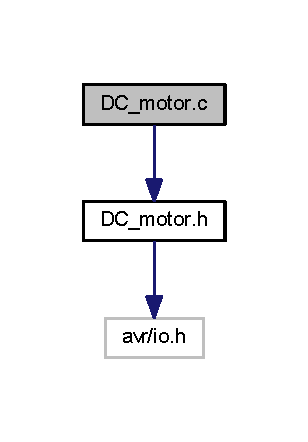
\includegraphics[width=148pt]{d9/d0e/_d_c__motor_8c__incl}
\end{center}
\end{figure}
\subsection*{Functions}
\begin{DoxyCompactItemize}
\item 
void \hyperlink{_d_c__motor_8c_a0f5ba92ac90e43a822ddc73547c361fd}{T\+I\+M\+E\+R0\+\_\+\+P\+WM} (char duty\+Cycle)
\item 
void \hyperlink{_d_c__motor_8c_af153a476821fc273ea3401a7cdd1e546}{motor\+\_\+dir} (char dir)
\end{DoxyCompactItemize}


\subsection{Function Documentation}
\mbox{\Hypertarget{_d_c__motor_8c_af153a476821fc273ea3401a7cdd1e546}\label{_d_c__motor_8c_af153a476821fc273ea3401a7cdd1e546}} 
\index{D\+C\+\_\+motor.\+c@{D\+C\+\_\+motor.\+c}!motor\+\_\+dir@{motor\+\_\+dir}}
\index{motor\+\_\+dir@{motor\+\_\+dir}!D\+C\+\_\+motor.\+c@{D\+C\+\_\+motor.\+c}}
\subsubsection{\texorpdfstring{motor\+\_\+dir()}{motor\_dir()}}
{\footnotesize\ttfamily void motor\+\_\+dir (\begin{DoxyParamCaption}\item[{char}]{dir }\end{DoxyParamCaption})}

\mbox{\Hypertarget{_d_c__motor_8c_a0f5ba92ac90e43a822ddc73547c361fd}\label{_d_c__motor_8c_a0f5ba92ac90e43a822ddc73547c361fd}} 
\index{D\+C\+\_\+motor.\+c@{D\+C\+\_\+motor.\+c}!T\+I\+M\+E\+R0\+\_\+\+P\+WM@{T\+I\+M\+E\+R0\+\_\+\+P\+WM}}
\index{T\+I\+M\+E\+R0\+\_\+\+P\+WM@{T\+I\+M\+E\+R0\+\_\+\+P\+WM}!D\+C\+\_\+motor.\+c@{D\+C\+\_\+motor.\+c}}
\subsubsection{\texorpdfstring{T\+I\+M\+E\+R0\+\_\+\+P\+W\+M()}{TIMER0\_PWM()}}
{\footnotesize\ttfamily void T\+I\+M\+E\+R0\+\_\+\+P\+WM (\begin{DoxyParamCaption}\item[{char}]{duty\+Cycle }\end{DoxyParamCaption})}


\hypertarget{_d_c__motor_8h}{}\section{D\+C\+\_\+motor.\+h File Reference}
\label{_d_c__motor_8h}\index{D\+C\+\_\+motor.\+h@{D\+C\+\_\+motor.\+h}}
{\ttfamily \#include $<$avr/io.\+h$>$}\newline
Include dependency graph for D\+C\+\_\+motor.\+h\+:\nopagebreak
\begin{figure}[H]
\begin{center}
\leavevmode
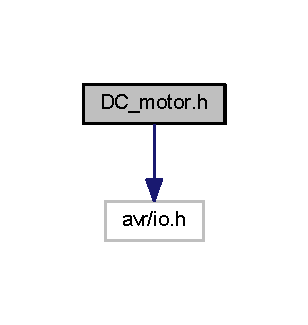
\includegraphics[width=148pt]{d5/d0b/_d_c__motor_8h__incl}
\end{center}
\end{figure}
This graph shows which files directly or indirectly include this file\+:\nopagebreak
\begin{figure}[H]
\begin{center}
\leavevmode
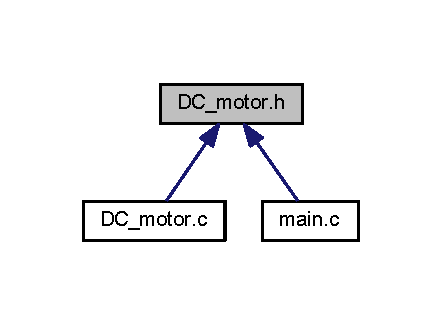
\includegraphics[width=212pt]{d6/d36/_d_c__motor_8h__dep__incl}
\end{center}
\end{figure}
\subsection*{Macros}
\begin{DoxyCompactItemize}
\item 
\#define \hyperlink{_d_c__motor_8h_a8a460b6555077a64fc97f2e7ef47b843}{C\+CW}~0
\item 
\#define \hyperlink{_d_c__motor_8h_abe61b07c31c2a3e90576eb4c5d95b024}{CW}~1
\end{DoxyCompactItemize}
\subsection*{Functions}
\begin{DoxyCompactItemize}
\item 
void \hyperlink{_d_c__motor_8h_a0f5ba92ac90e43a822ddc73547c361fd}{T\+I\+M\+E\+R0\+\_\+\+P\+WM} (char duty\+Cycle)
\item 
void \hyperlink{_d_c__motor_8h_af153a476821fc273ea3401a7cdd1e546}{motor\+\_\+dir} (char dir)
\end{DoxyCompactItemize}


\subsection{Macro Definition Documentation}
\mbox{\Hypertarget{_d_c__motor_8h_a8a460b6555077a64fc97f2e7ef47b843}\label{_d_c__motor_8h_a8a460b6555077a64fc97f2e7ef47b843}} 
\index{D\+C\+\_\+motor.\+h@{D\+C\+\_\+motor.\+h}!C\+CW@{C\+CW}}
\index{C\+CW@{C\+CW}!D\+C\+\_\+motor.\+h@{D\+C\+\_\+motor.\+h}}
\subsubsection{\texorpdfstring{C\+CW}{CCW}}
{\footnotesize\ttfamily \#define C\+CW~0}

\mbox{\Hypertarget{_d_c__motor_8h_abe61b07c31c2a3e90576eb4c5d95b024}\label{_d_c__motor_8h_abe61b07c31c2a3e90576eb4c5d95b024}} 
\index{D\+C\+\_\+motor.\+h@{D\+C\+\_\+motor.\+h}!CW@{CW}}
\index{CW@{CW}!D\+C\+\_\+motor.\+h@{D\+C\+\_\+motor.\+h}}
\subsubsection{\texorpdfstring{CW}{CW}}
{\footnotesize\ttfamily \#define CW~1}



\subsection{Function Documentation}
\mbox{\Hypertarget{_d_c__motor_8h_af153a476821fc273ea3401a7cdd1e546}\label{_d_c__motor_8h_af153a476821fc273ea3401a7cdd1e546}} 
\index{D\+C\+\_\+motor.\+h@{D\+C\+\_\+motor.\+h}!motor\+\_\+dir@{motor\+\_\+dir}}
\index{motor\+\_\+dir@{motor\+\_\+dir}!D\+C\+\_\+motor.\+h@{D\+C\+\_\+motor.\+h}}
\subsubsection{\texorpdfstring{motor\+\_\+dir()}{motor\_dir()}}
{\footnotesize\ttfamily void motor\+\_\+dir (\begin{DoxyParamCaption}\item[{char}]{dir }\end{DoxyParamCaption})}

\mbox{\Hypertarget{_d_c__motor_8h_a0f5ba92ac90e43a822ddc73547c361fd}\label{_d_c__motor_8h_a0f5ba92ac90e43a822ddc73547c361fd}} 
\index{D\+C\+\_\+motor.\+h@{D\+C\+\_\+motor.\+h}!T\+I\+M\+E\+R0\+\_\+\+P\+WM@{T\+I\+M\+E\+R0\+\_\+\+P\+WM}}
\index{T\+I\+M\+E\+R0\+\_\+\+P\+WM@{T\+I\+M\+E\+R0\+\_\+\+P\+WM}!D\+C\+\_\+motor.\+h@{D\+C\+\_\+motor.\+h}}
\subsubsection{\texorpdfstring{T\+I\+M\+E\+R0\+\_\+\+P\+W\+M()}{TIMER0\_PWM()}}
{\footnotesize\ttfamily void T\+I\+M\+E\+R0\+\_\+\+P\+WM (\begin{DoxyParamCaption}\item[{char}]{duty\+Cycle }\end{DoxyParamCaption})}


\hypertarget{main_8c}{}\section{main.\+c File Reference}
\label{main_8c}\index{main.\+c@{main.\+c}}


This is the main file of the project.  


{\ttfamily \#include $<$avr/io.\+h$>$}\newline
{\ttfamily \#include \char`\"{}U\+A\+R\+T.\+h\char`\"{}}\newline
{\ttfamily \#include \char`\"{}D\+C\+\_\+motor.\+h\char`\"{}}\newline
{\ttfamily \#include \char`\"{}Servo.\+h\char`\"{}}\newline
Include dependency graph for main.\+c\+:
\nopagebreak
\begin{figure}[H]
\begin{center}
\leavevmode
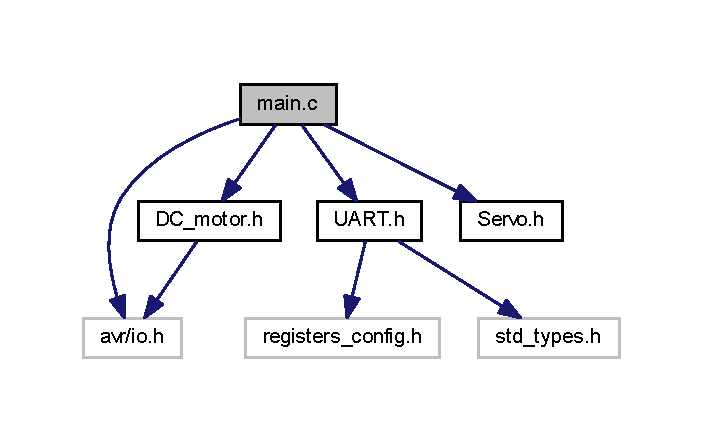
\includegraphics[width=338pt]{d4/d10/main_8c__incl}
\end{center}
\end{figure}
\subsection*{Functions}
\begin{DoxyCompactItemize}
\item 
int \hyperlink{main_8c_a840291bc02cba5474a4cb46a9b9566fe}{main} (void)
\end{DoxyCompactItemize}


\subsection{Detailed Description}
This is the main file of the project. 

\begin{DoxyAuthor}{Author}
Hardware Sub\+Group 
\end{DoxyAuthor}
\begin{DoxyDate}{Date}
1 Dec 2017 
\end{DoxyDate}


\subsection{Function Documentation}
\mbox{\Hypertarget{main_8c_a840291bc02cba5474a4cb46a9b9566fe}\label{main_8c_a840291bc02cba5474a4cb46a9b9566fe}} 
\index{main.\+c@{main.\+c}!main@{main}}
\index{main@{main}!main.\+c@{main.\+c}}
\subsubsection{\texorpdfstring{main()}{main()}}
{\footnotesize\ttfamily int main (\begin{DoxyParamCaption}\item[{void}]{ }\end{DoxyParamCaption})}


\hypertarget{_servo_8c}{}\section{Servo.\+c File Reference}
\label{_servo_8c}\index{Servo.\+c@{Servo.\+c}}
{\ttfamily \#include \char`\"{}Servo.\+h\char`\"{}}\newline
Include dependency graph for Servo.\+c\+:
\nopagebreak
\begin{figure}[H]
\begin{center}
\leavevmode
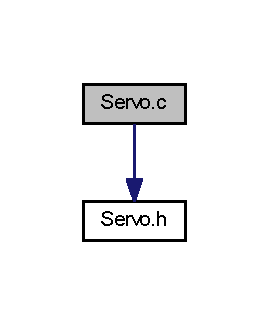
\includegraphics[width=129pt]{de/d38/_servo_8c__incl}
\end{center}
\end{figure}
\subsection*{Functions}
\begin{DoxyCompactItemize}
\item 
void \hyperlink{_servo_8c_a8dff2a30f0ed2637f09a71a2b1cf9d9e}{servo\+\_\+\+Init} ()
\item 
void \hyperlink{_servo_8c_a5cfd960b255b24456f57e7be522a7e22}{servo\+\_\+\+S\+T\+EP} (uint8 angle)
\end{DoxyCompactItemize}


\subsection{Function Documentation}
\mbox{\Hypertarget{_servo_8c_a8dff2a30f0ed2637f09a71a2b1cf9d9e}\label{_servo_8c_a8dff2a30f0ed2637f09a71a2b1cf9d9e}} 
\index{Servo.\+c@{Servo.\+c}!servo\+\_\+\+Init@{servo\+\_\+\+Init}}
\index{servo\+\_\+\+Init@{servo\+\_\+\+Init}!Servo.\+c@{Servo.\+c}}
\subsubsection{\texorpdfstring{servo\+\_\+\+Init()}{servo\_Init()}}
{\footnotesize\ttfamily void servo\+\_\+\+Init (\begin{DoxyParamCaption}{ }\end{DoxyParamCaption})}

\mbox{\Hypertarget{_servo_8c_a5cfd960b255b24456f57e7be522a7e22}\label{_servo_8c_a5cfd960b255b24456f57e7be522a7e22}} 
\index{Servo.\+c@{Servo.\+c}!servo\+\_\+\+S\+T\+EP@{servo\+\_\+\+S\+T\+EP}}
\index{servo\+\_\+\+S\+T\+EP@{servo\+\_\+\+S\+T\+EP}!Servo.\+c@{Servo.\+c}}
\subsubsection{\texorpdfstring{servo\+\_\+\+S\+T\+E\+P()}{servo\_STEP()}}
{\footnotesize\ttfamily void servo\+\_\+\+S\+T\+EP (\begin{DoxyParamCaption}\item[{uint8}]{angle }\end{DoxyParamCaption})}


\hypertarget{_servo_8h}{}\section{Servo.\+h File Reference}
\label{_servo_8h}\index{Servo.\+h@{Servo.\+h}}


this is the library to control the servo motor  


{\ttfamily \#include \char`\"{}micro\+\_\+config.\+h\char`\"{}}\newline
{\ttfamily \#include \char`\"{}std\+\_\+types.\+h\char`\"{}}\newline
{\ttfamily \#include \char`\"{}common\+\_\+macros.\+h\char`\"{}}\newline
Include dependency graph for Servo.\+h\+:\nopagebreak
\begin{figure}[H]
\begin{center}
\leavevmode
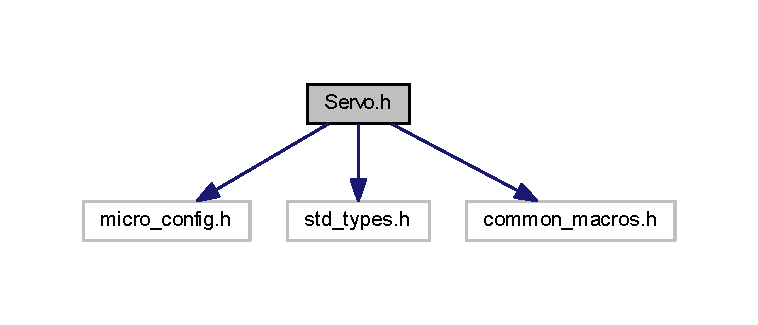
\includegraphics[width=350pt]{_servo_8h__incl}
\end{center}
\end{figure}
This graph shows which files directly or indirectly include this file\+:\nopagebreak
\begin{figure}[H]
\begin{center}
\leavevmode
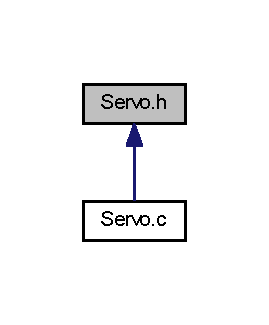
\includegraphics[width=129pt]{_servo_8h__dep__incl}
\end{center}
\end{figure}
\subsection*{Functions}
\begin{DoxyCompactItemize}
\item 
void \hyperlink{_servo_8h_a8dff2a30f0ed2637f09a71a2b1cf9d9e}{servo\+\_\+\+Init} ()
\item 
void \hyperlink{_servo_8h_a5cfd960b255b24456f57e7be522a7e22}{servo\+\_\+\+S\+T\+EP} (uint8 angle)
\end{DoxyCompactItemize}


\subsection{Detailed Description}
this is the library to control the servo motor 



\subsection{Function Documentation}
\mbox{\Hypertarget{_servo_8h_a8dff2a30f0ed2637f09a71a2b1cf9d9e}\label{_servo_8h_a8dff2a30f0ed2637f09a71a2b1cf9d9e}} 
\index{Servo.\+h@{Servo.\+h}!servo\+\_\+\+Init@{servo\+\_\+\+Init}}
\index{servo\+\_\+\+Init@{servo\+\_\+\+Init}!Servo.\+h@{Servo.\+h}}
\subsubsection{\texorpdfstring{servo\+\_\+\+Init()}{servo\_Init()}}
{\footnotesize\ttfamily void servo\+\_\+\+Init (\begin{DoxyParamCaption}{ }\end{DoxyParamCaption})}

\mbox{\Hypertarget{_servo_8h_a5cfd960b255b24456f57e7be522a7e22}\label{_servo_8h_a5cfd960b255b24456f57e7be522a7e22}} 
\index{Servo.\+h@{Servo.\+h}!servo\+\_\+\+S\+T\+EP@{servo\+\_\+\+S\+T\+EP}}
\index{servo\+\_\+\+S\+T\+EP@{servo\+\_\+\+S\+T\+EP}!Servo.\+h@{Servo.\+h}}
\subsubsection{\texorpdfstring{servo\+\_\+\+S\+T\+E\+P()}{servo\_STEP()}}
{\footnotesize\ttfamily void servo\+\_\+\+S\+T\+EP (\begin{DoxyParamCaption}\item[{uint8}]{angle }\end{DoxyParamCaption})}


\hypertarget{_u_a_r_t_01_8c}{}\section{U\+A\+RT .c File Reference}
\label{_u_a_r_t_01_8c}\index{U\+A\+R\+T .\+c@{U\+A\+R\+T .\+c}}
{\ttfamily \#include \char`\"{}U\+A\+R\+T.\+h\char`\"{}}\newline
Include dependency graph for U\+A\+RT .c\+:
\nopagebreak
\begin{figure}[H]
\begin{center}
\leavevmode
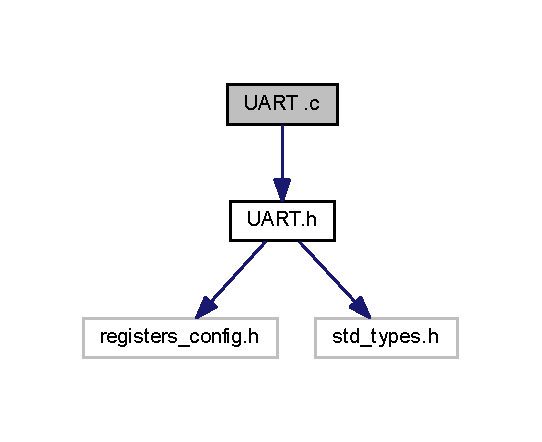
\includegraphics[width=260pt]{_u_a_r_t_01_8c__incl}
\end{center}
\end{figure}
\subsection*{Functions}
\begin{DoxyCompactItemize}
\item 
void \hyperlink{_u_a_r_t_01_8c_afbfe9a19c497ec9e0586c7e6feb4897a}{uart\+\_\+init} (uint8 uart\+\_\+num)
\begin{DoxyCompactList}\small\item\em U\+A\+RT initialization \+: ~\newline
Tiva c has 8 channels for uart so the variable uart\+\_\+num is the channel number. \end{DoxyCompactList}\item 
void \hyperlink{_u_a_r_t_01_8c_ab0d6a19096405d3f0e1a47da77093c59}{uart\+\_\+send\+\_\+byte} (uint8 uart\+\_\+num, uint8 data)
\begin{DoxyCompactList}\small\item\em send a byte to other device \+: ~\newline
variable uart\+\_\+num for channel number specified before ~\newline
variable data for the desired data to be sent ~\newline
\end{DoxyCompactList}\item 
uint8 \hyperlink{_u_a_r_t_01_8c_a6672b250ddc566fa64e11ffb6d264048}{uart\+\_\+recieve\+\_\+byte} (uint8 uart\+\_\+num)
\begin{DoxyCompactList}\small\item\em receive a byte from other device \+: ~\newline
variable uart\+\_\+num is for the channel number specified before \end{DoxyCompactList}\end{DoxyCompactItemize}


\subsection{Function Documentation}
\mbox{\Hypertarget{_u_a_r_t_01_8c_afbfe9a19c497ec9e0586c7e6feb4897a}\label{_u_a_r_t_01_8c_afbfe9a19c497ec9e0586c7e6feb4897a}} 
\index{U\+A\+R\+T .\+c@{U\+A\+R\+T .\+c}!uart\+\_\+init@{uart\+\_\+init}}
\index{uart\+\_\+init@{uart\+\_\+init}!U\+A\+R\+T .\+c@{U\+A\+R\+T .\+c}}
\subsubsection{\texorpdfstring{uart\+\_\+init()}{uart\_init()}}
{\footnotesize\ttfamily void uart\+\_\+init (\begin{DoxyParamCaption}\item[{uint8}]{uart\+\_\+num }\end{DoxyParamCaption})}



U\+A\+RT initialization \+: ~\newline
Tiva c has 8 channels for uart so the variable uart\+\_\+num is the channel number. 


\begin{DoxyCode}
      \textcolor{keywordflow}{if}(uart\_num == 0)
\{
    \textcolor{keyword}{volatile} uint32 delay;
    \textcolor{comment}{/* Assumes a 16 MHz bus clock, creates 9600 baud rate */}

    \textcolor{comment}{/* Enable and provide a clock to UART module in Run mode */}
    SYSCTL\_RCGC1\_R |=(1<<uart\_num);

    \textcolor{comment}{/* allow time to finish activating */}
    delay = SYSCTL\_RCGC2\_R;

    \textcolor{comment}{/* SYSCTL\_RCGCGPIO\_R enabled by function ports\_clock\_EN() for all ports */}

    \textcolor{comment}{/*  disable UART */}
    UART0\_CTL\_R &= ~(0x00000001);

    \textcolor{comment}{/* Set the GPIO AFSEL bits to enable alternative function */}
    GPIO\_PORTA\_AFSEL\_R |= 0x03 ;

    \textcolor{comment}{/* Configure the PMCn fields in the GPIOPCTL register to assign the UART signals */}
    GPIO\_PORTA\_PCTL\_R = (GPIO\_PORTA\_PCTL\_R & 0xFFFFFF00) | (0x00000011) ;



    \textcolor{comment}{/* IBRD = int(16,000,000/(16*9600)) = int(104.1666667) */}
    UART0\_IBRD\_R = 104;

    \textcolor{comment}{/* UARTFBRD[DIVFRAC] = integer(0.166666667 * 64 + 0.5) = int(11.1666) = 11 */}
    UART0\_FBRD\_R = 11;

    \textcolor{comment}{/*  8 bit, no parity bits, one stop, disable FIFOs */}
    UART0\_LCRH\_R |= 0x00000060;

    \textcolor{comment}{/* enable UART */}
    UART0\_CTL\_R |= 0x00000301;

    \textcolor{comment}{/* The digital functions for the corresponding pin are enabled */}
    GPIO\_PORTA\_DEN\_R |= 0X03;

    \textcolor{comment}{/* disable analog on pins */}
    GPIO\_PORTA\_AMSEL\_R &= ~(0x03);
\}

\textcolor{keywordflow}{else} \textcolor{keywordflow}{if}(uart\_num == 1)
\{
    \textcolor{keyword}{volatile} uint32 delay;
    \textcolor{comment}{/* Assumes a 80 MHz bus clock, creates 9600 baud rate */}

    \textcolor{comment}{/* Enable and provide a clock to UART module in Run mode */}
    SYSCTL\_RCGC1\_R |=(1<<uart\_num);

    \textcolor{comment}{/* allow time to finish activating */}
    delay = SYSCTL\_RCGC2\_R;

    \textcolor{comment}{/* SYSCTL\_RCGCGPIO\_R enabled by function ports\_clock\_EN() for all ports */}

    \textcolor{comment}{/*  disable UART */}
    UART1\_CTL\_R &= ~(0x00000001);

    \textcolor{comment}{/* Set the GPIO AFSEL bits to enable alt funct */}
    GPIO\_PORTB\_AFSEL\_R |= 0x03 ;

    \textcolor{comment}{/* Configure the PMCn fields in the GPIOPCTL register to assign the UART signals */}
    GPIO\_PORTB\_PCTL\_R = (GPIO\_PORTA\_PCTL\_R & 0xFFFFFF00) | (0x00000011) ;



    \textcolor{comment}{/* IBRD = int(16,000,000/(16*9600)) = int(104.1666667) */}
    UART1\_IBRD\_R = 104;

    \textcolor{comment}{/* UARTFBRD[DIVFRAC] = integer(0.166666667 * 64 + 0.5) = int(11.1666) = 11 */}
    UART1\_FBRD\_R = 11;

    \textcolor{comment}{/*  8 bit, no parity bits, one stop, disable FIFOs */}
    UART1\_LCRH\_R |= 0x00000060;

    \textcolor{comment}{/* enable UART */}
    UART1\_CTL\_R |= 0x00000301;

    \textcolor{comment}{/* The digital functions for the corresponding pin are enabled */}
    GPIO\_PORTB\_DEN\_R |= 0X03;

    \textcolor{comment}{/* disable analog on pins */}
    GPIO\_PORTB\_AMSEL\_R &= ~(0x03);

\}
\textcolor{keywordflow}{else} \textcolor{keywordflow}{if}(uart\_num == 2)
\{
    \textcolor{keyword}{volatile} uint32 delay;
    \textcolor{comment}{/* Assumes a 80 MHz bus clock, creates 9600 baud rate */}

    \textcolor{comment}{/* Enable and provide a clock to UART module in Run mode */}
    SYSCTL\_RCGC1\_R |=(1<<uart\_num);

    \textcolor{comment}{/* allow time to finish activating */}
    delay = SYSCTL\_RCGC2\_R;

    \textcolor{comment}{/* SYSCTL\_RCGCGPIO\_R enabled by function ports\_clock\_EN() for all ports */}

    \textcolor{comment}{/*  disable UART */}
    UART2\_CTL\_R &= ~(0x00000001);

    \textcolor{comment}{/* Set the GPIO AFSEL bits to enable alternative function */}
    GPIO\_PORTD\_AFSEL\_R |= 0xC0 ;

    \textcolor{comment}{/* Configure the PMCn fields in the GPIOPCTL register to assign the UART signals */}
    GPIO\_PORTD\_PCTL\_R = (GPIO\_PORTA\_PCTL\_R & 0x00FFFFFF) | (0x11000000) ;

    \textcolor{comment}{/* IBRD = int(16,000,000/(16*9600)) = int(104.1666667) */}
    UART2\_IBRD\_R = 104;

    \textcolor{comment}{/* UARTFBRD[DIVFRAC] = integer(0.166666667 * 64 + 0.5) = int(11.1666) = 11 */}
    UART2\_FBRD\_R = 11;

    \textcolor{comment}{/*  8 bit, no parity bits, one stop, disable FIFOs */}
    UART2\_LCRH\_R |= 0x00000060;

    \textcolor{comment}{/* enable UART */}
    UART2\_CTL\_R |= 0x00000301;

    \textcolor{comment}{/* The digital functions for the corresponding pin are enabled */}
    GPIO\_PORTD\_DEN\_R |= 0XC0;

    \textcolor{comment}{/* disable analog on pins */}
    GPIO\_PORTD\_AMSEL\_R &= ~(0xC0);

\}

\textcolor{keywordflow}{else} \textcolor{keywordflow}{if}(uart\_num == 3)
\{
    \textcolor{keyword}{volatile} uint32 delay;
    \textcolor{comment}{/* Assumes a 80 MHz bus clock, creates 9600 baud rate */}

    \textcolor{comment}{/* Enable and provide a clock to UART module in Run mode */}
    SYSCTL\_RCGC1\_R |=(1<<uart\_num);

    \textcolor{comment}{/* allow time to finish activating */}
    delay = SYSCTL\_RCGC2\_R;

    \textcolor{comment}{/* SYSCTL\_RCGCGPIO\_R enabled by function ports\_clock\_EN() for all ports */}

    \textcolor{comment}{/*  disable UART */}
    UART3\_CTL\_R &= ~(0x00000001);

    \textcolor{comment}{/* Set the GPIO AFSEL bits to enable alternative function */}
    GPIO\_PORTC\_AFSEL\_R |= 0xC0 ;

    \textcolor{comment}{/* Configure the PMCn fields in the GPIOPCTL register to assign the UART signals */}
    GPIO\_PORTC\_PCTL\_R = (GPIO\_PORTA\_PCTL\_R & 0x00FFFFFF) | (0x11000000) ;

    \textcolor{comment}{/* IBRD = int(16,000,000/(16*9600)) = int(104.1666667) */}
    UART3\_IBRD\_R = 104;

    \textcolor{comment}{/* UARTFBRD[DIVFRAC] = integer(0.166666667 * 64 + 0.5) = int(11.1666) = 11 */}
    UART3\_FBRD\_R = 11;

    \textcolor{comment}{/*  8 bit, no parity bits, one stop, disable FIFOs */}
    UART3\_LCRH\_R |= 0x00000060;

    \textcolor{comment}{/* enable UART */}
    UART3\_CTL\_R |= 0x00000301;

    \textcolor{comment}{/* The digital functions for the corresponding pin are enabled */}
    GPIO\_PORTC\_DEN\_R |= 0XC0;

    \textcolor{comment}{/* disable analog on pins */}
    GPIO\_PORTC\_AMSEL\_R &= ~(0xC0);

\}

\textcolor{keywordflow}{else} \textcolor{keywordflow}{if}(uart\_num == 4)
\{
    \textcolor{keyword}{volatile} uint32 delay;
    \textcolor{comment}{/* Assumes a 80 MHz bus clock, creates 9600 baud rate */}

    \textcolor{comment}{/* Enable and provide a clock to UART module in Run mode */}
    SYSCTL\_RCGC1\_R |=(1<<uart\_num);

    \textcolor{comment}{/* allow time to finish activating */}
    delay = SYSCTL\_RCGC2\_R;


    \textcolor{comment}{/* SYSCTL\_RCGCGPIO\_R enabled by function ports\_clock\_EN() for all ports */}

    \textcolor{comment}{/*  disable UART */}
    UART4\_CTL\_R &= ~(0x00000001);

    \textcolor{comment}{/* Set the GPIO AFSEL bits to enable alternative function */}
    GPIO\_PORTC\_AFSEL\_R |= 0x30 ;

    \textcolor{comment}{/* Configure the PMCn fields in the GPIOPCTL register to assign the UART signals */}
    GPIO\_PORTC\_PCTL\_R = (GPIO\_PORTA\_PCTL\_R & 0xFF00FFFF) | (0x00110000) ;

    \textcolor{comment}{/* IBRD = int(16,000,000/(16*9600)) = int(104.1666667) */}
    UART4\_IBRD\_R = 104;

    \textcolor{comment}{/* UARTFBRD[DIVFRAC] = integer(0.166666667 * 64 + 0.5) = int(11.1666) = 11 */}
    UART4\_FBRD\_R = 11;

    \textcolor{comment}{/*  8 bit, no parity bits, one stop, disable FIFOs */}
    UART4\_LCRH\_R |= 0x00000060;

    \textcolor{comment}{/* enable UART */}
    UART4\_CTL\_R |= 0x00000301;

    \textcolor{comment}{/* The digital functions for the corresponding pin are enabled */}
    GPIO\_PORTC\_DEN\_R |= 0X30;

    \textcolor{comment}{/* disable analog on pins */}
    GPIO\_PORTC\_AMSEL\_R &= ~(0x30);

\}

\textcolor{keywordflow}{else} \textcolor{keywordflow}{if}(uart\_num == 5)
\{
    \textcolor{keyword}{volatile} uint32 delay;
    \textcolor{comment}{/* Assumes a 80 MHz bus clock, creates 9600 baud rate */}

    \textcolor{comment}{/* Enable and provide a clock to UART module in Run mode */}
    SYSCTL\_RCGC1\_R |=(1<<uart\_num);

    \textcolor{comment}{/* allow time to finish activating */}
    delay = SYSCTL\_RCGC2\_R;


    \textcolor{comment}{/* SYSCTL\_RCGCGPIO\_R enabled by function ports\_clock\_EN() for all ports */}

    \textcolor{comment}{/*  disable UART */}
    UART5\_CTL\_R &= ~(0x00000001);

    \textcolor{comment}{/* Set the GPIO AFSEL bits to enable alternative function */}
    GPIO\_PORTE\_AFSEL\_R |= 0x03 ;

    \textcolor{comment}{/* Configure the PMCn fields in the GPIOPCTL register to assign the UART signals */}
    GPIO\_PORTE\_PCTL\_R = (GPIO\_PORTA\_PCTL\_R & 0xFFFFFF00) | (0x00000011) ;

    \textcolor{comment}{/* IBRD = int(16,000,000/(16*9600)) = int(104.1666667) */}
    UART5\_IBRD\_R = 104;

    \textcolor{comment}{/* UARTFBRD[DIVFRAC] = integer(0.166666667 * 64 + 0.5) = int(11.1666) = 11 */}
    UART5\_FBRD\_R = 11;

    \textcolor{comment}{/*  8 bit, no parity bits, one stop, disable FIFOs */}
    UART5\_LCRH\_R |= 0x00000060;

    \textcolor{comment}{/* enable UART */}
    UART5\_CTL\_R |= 0x00000301;

    \textcolor{comment}{/* The digital functions for the corresponding pin are enabled */}
    GPIO\_PORTE\_DEN\_R |= 0X03;

    \textcolor{comment}{/* disable analog on pins */}
    GPIO\_PORTE\_AMSEL\_R &= ~(0x03);

\}

\textcolor{keywordflow}{else} \textcolor{keywordflow}{if}(uart\_num == 6)
\{
    \textcolor{keyword}{volatile} uint32 delay;
    \textcolor{comment}{/* Assumes a 80 MHz bus clock, creates 9600 baud rate */}

    \textcolor{comment}{/* Enable and provide a clock to UART module in Run mode */}
    SYSCTL\_RCGC1\_R |=(1<<uart\_num);

    \textcolor{comment}{/* allow time to finish activating */}
    delay = SYSCTL\_RCGC2\_R;

    \textcolor{comment}{/* SYSCTL\_RCGCGPIO\_R enabled by function ports\_clock\_EN() for all ports */}

    \textcolor{comment}{/*  disable UART */}
    UART6\_CTL\_R &= ~(0x00000001);

    \textcolor{comment}{/* Set the GPIO AFSEL bits to enable alternative function */}
    GPIO\_PORTD\_AFSEL\_R |= 0x30 ;

    \textcolor{comment}{/* Configure the PMCn fields in the GPIOPCTL register to assign the UART signals */}
    GPIO\_PORTD\_PCTL\_R = (GPIO\_PORTA\_PCTL\_R & 0xFF00FFFF) | (0x00110000) ;

    \textcolor{comment}{/* IBRD = int(16,000,000/(16*9600)) = int(104.1666667) */}
    UART6\_IBRD\_R = 104;

    \textcolor{comment}{/* UARTFBRD[DIVFRAC] = integer(0.166666667 * 64 + 0.5) = int(11.1666) = 11 */}
    UART6\_FBRD\_R = 11;

    \textcolor{comment}{/*  8 bit, no parity bits, one stop, disable FIFOs */}
    UART6\_LCRH\_R |= 0x00000060;

    \textcolor{comment}{/* enable UART */}
    UART6\_CTL\_R |= 0x00000301;

    \textcolor{comment}{/* The digital functions for the corresponding pin are enabled */}
    GPIO\_PORTD\_DEN\_R |= 0X30;

    \textcolor{comment}{/* disable analog on pins */}
    GPIO\_PORTD\_AMSEL\_R &= ~(0x30);

\}

\textcolor{keywordflow}{else} \textcolor{keywordflow}{if}(uart\_num == 7)
\{
    \textcolor{keyword}{volatile} uint32 delay;
    \textcolor{comment}{/* Assumes a 80 MHz bus clock, creates 9600 baud rate */}

    \textcolor{comment}{/* Enable and provide a clock to UART module in Run mode */}
    SYSCTL\_RCGC1\_R |=(1<<uart\_num);

    \textcolor{comment}{/* allow time to finish activating */}
    delay = SYSCTL\_RCGC2\_R;

    \textcolor{comment}{/* SYSCTL\_RCGCGPIO\_R enabled by function ports\_clock\_EN() for all ports */}

    \textcolor{comment}{/*  disable UART */}
    UART7\_CTL\_R &= ~(0x00000001);

    \textcolor{comment}{/* Set the GPIO AFSEL bits to enable alternative function */}
    GPIO\_PORTE\_AFSEL\_R |= 0x03 ;

    \textcolor{comment}{/* Configure the PMCn fields in the GPIOPCTL register to assign the UART signals */}
    GPIO\_PORTE\_PCTL\_R = (GPIO\_PORTA\_PCTL\_R & 0xFFFFFF00) | (0x00000011) ;

    \textcolor{comment}{/* IBRD = int(16,000,000/(16*9600)) = int(104.1666667) */}
    UART7\_IBRD\_R = 104;

    \textcolor{comment}{/* UARTFBRD[DIVFRAC] = integer(0.166666667 * 64 + 0.5) = int(11.1666) = 11 */}
    UART7\_FBRD\_R = 11;

    \textcolor{comment}{/*  8 bit, no parity bits, one stop, disable FIFOs */}
    UART7\_LCRH\_R |= 0x00000060;

    \textcolor{comment}{/* enable UART */}
    UART7\_CTL\_R |= 0x00000301;

    \textcolor{comment}{/* The digital functions for the corresponding pin are enabled */}
    GPIO\_PORTE\_DEN\_R |= 0X03;

    \textcolor{comment}{/* disable analog on pins */}
    GPIO\_PORTE\_AMSEL\_R &= ~(0x03);

\}


\}
\end{DoxyCode}
 \mbox{\Hypertarget{_u_a_r_t_01_8c_a6672b250ddc566fa64e11ffb6d264048}\label{_u_a_r_t_01_8c_a6672b250ddc566fa64e11ffb6d264048}} 
\index{U\+A\+R\+T .\+c@{U\+A\+R\+T .\+c}!uart\+\_\+recieve\+\_\+byte@{uart\+\_\+recieve\+\_\+byte}}
\index{uart\+\_\+recieve\+\_\+byte@{uart\+\_\+recieve\+\_\+byte}!U\+A\+R\+T .\+c@{U\+A\+R\+T .\+c}}
\subsubsection{\texorpdfstring{uart\+\_\+recieve\+\_\+byte()}{uart\_recieve\_byte()}}
{\footnotesize\ttfamily uint8 uart\+\_\+recieve\+\_\+byte (\begin{DoxyParamCaption}\item[{uint8}]{uart\+\_\+num }\end{DoxyParamCaption})}



receive a byte from other device \+: ~\newline
variable uart\+\_\+num is for the channel number specified before 


\begin{DoxyCode}
 \{
    \textcolor{comment}{/* function to recieve byte takes one input (uart number)}
\textcolor{comment}{     * return recieved byte  */}

    \textcolor{keywordflow}{if}(uart\_num == 0)
    \{
        \textcolor{comment}{/* Wait for new input ,wait until RXFE is 0 */}
        \textcolor{keywordflow}{while}((UART0\_FR\_R & 0x0010) != 0);
        \textcolor{keywordflow}{return} ((uint8)(UART0\_DR\_R & 0xFF)) ;

    \}

    \textcolor{keywordflow}{else} \textcolor{keywordflow}{if}(uart\_num == 1)
    \{
        \textcolor{comment}{/* Wait for new input ,wait until RXFE is 0 */}
        \textcolor{keywordflow}{while}((UART1\_FR\_R & 0x0010) != 0)\{\}
        \textcolor{keywordflow}{return} ((uint8)(UART1\_DR\_R & 0xFF)) ;
    \}

    \textcolor{keywordflow}{else} \textcolor{keywordflow}{if}(uart\_num == 2)
    \{
        \textcolor{comment}{/* Wait for new input ,wait until RXFE is 0 */}
        \textcolor{keywordflow}{while}((UART2\_FR\_R & 0x0010) != 0);
        \textcolor{keywordflow}{return} ((uint8)(UART2\_DR\_R & 0xFF)) ;
    \}

    \textcolor{keywordflow}{else} \textcolor{keywordflow}{if}(uart\_num == 3)
    \{
        \textcolor{comment}{/* Wait for new input ,wait until RXFE is 0 */}
        \textcolor{keywordflow}{while}((UART3\_FR\_R & 0x0010) != 0);
        \textcolor{keywordflow}{return} ((uint8)(UART3\_DR\_R & 0xFF)) ;
    \}

    \textcolor{keywordflow}{else} \textcolor{keywordflow}{if}(uart\_num == 4)
    \{
        \textcolor{comment}{/* Wait for new input ,wait until RXFE is 0 */}
        \textcolor{keywordflow}{while}((UART4\_FR\_R & 0x0010) != 0);
        \textcolor{keywordflow}{return} ((uint8)(UART4\_DR\_R & 0xFF)) ;
    \}

    \textcolor{keywordflow}{else} \textcolor{keywordflow}{if}(uart\_num == 5)
    \{
        \textcolor{comment}{/* Wait for new input ,wait until RXFE is 0 */}
        \textcolor{keywordflow}{while}((UART5\_FR\_R & 0x0010) != 0);
        \textcolor{keywordflow}{return} ((uint8)(UART5\_DR\_R & 0xFF)) ;
    \}

    \textcolor{keywordflow}{else} \textcolor{keywordflow}{if}(uart\_num == 6)
    \{
        \textcolor{comment}{/* Wait for new input ,wait until RXFE is 0 */}
        \textcolor{keywordflow}{while}((UART6\_FR\_R & 0x0010) != 0);
        \textcolor{keywordflow}{return} ((uint8)(UART6\_DR\_R & 0xFF)) ;
    \}

    \textcolor{keywordflow}{else} \textcolor{keywordflow}{if}(uart\_num == 7)
    \{
        \textcolor{comment}{/* Wait for new input ,wait until RXFE is 0 */}
        \textcolor{keywordflow}{while}((UART7\_FR\_R & 0x0010) != 0);
        \textcolor{keywordflow}{return} ((uint8)(UART7\_DR\_R & 0xFF)) ;
    \}


\}
\end{DoxyCode}
 \mbox{\Hypertarget{_u_a_r_t_01_8c_ab0d6a19096405d3f0e1a47da77093c59}\label{_u_a_r_t_01_8c_ab0d6a19096405d3f0e1a47da77093c59}} 
\index{U\+A\+R\+T .\+c@{U\+A\+R\+T .\+c}!uart\+\_\+send\+\_\+byte@{uart\+\_\+send\+\_\+byte}}
\index{uart\+\_\+send\+\_\+byte@{uart\+\_\+send\+\_\+byte}!U\+A\+R\+T .\+c@{U\+A\+R\+T .\+c}}
\subsubsection{\texorpdfstring{uart\+\_\+send\+\_\+byte()}{uart\_send\_byte()}}
{\footnotesize\ttfamily void uart\+\_\+send\+\_\+byte (\begin{DoxyParamCaption}\item[{uint8}]{uart\+\_\+num,  }\item[{uint8}]{data }\end{DoxyParamCaption})}



send a byte to other device \+: ~\newline
variable uart\+\_\+num for channel number specified before ~\newline
variable data for the desired data to be sent ~\newline



\begin{DoxyCode}
  \{
    \textcolor{comment}{/* void function to send byte takes data and uart number  */}
    \textcolor{keywordflow}{if}(uart\_num == 0)
    \{
        \textcolor{comment}{/* Wait for buffer to be not full ,TXFF to be clear */}
        \textcolor{keywordflow}{while}((UART0\_FR\_R & 0x0020) != 0)\{\}
        UART0\_DR\_R = data ;

    \}

    \textcolor{keywordflow}{else} \textcolor{keywordflow}{if}(uart\_num == 1)
    \{
        \textcolor{comment}{/* Wait for buffer to be not full ,TXFF to be clear */}
        \textcolor{keywordflow}{while}((UART1\_FR\_R & 0x0020) != 0)\{\}
        UART1\_DR\_R = data ;
    \}

    \textcolor{keywordflow}{else} \textcolor{keywordflow}{if}(uart\_num == 2)
    \{
        \textcolor{comment}{/* Wait for buffer to be not full ,TXFF to be clear */}
        \textcolor{keywordflow}{while}((UART2\_FR\_R & 0x0020) != 0);
        UART2\_DR\_R = data ;
    \}

    \textcolor{keywordflow}{else} \textcolor{keywordflow}{if}(uart\_num == 3)
    \{
        \textcolor{comment}{/* Wait for buffer to be not full ,TXFF to be clear */}
        \textcolor{keywordflow}{while}((UART3\_FR\_R & 0x0020) != 0);
        UART3\_DR\_R = data ;

    \}

    \textcolor{keywordflow}{else} \textcolor{keywordflow}{if}(uart\_num == 4)
    \{
        \textcolor{comment}{/* Wait for buffer to be not full ,TXFF to be clear */}
        \textcolor{keywordflow}{while}((UART4\_FR\_R & 0x0020) != 0);
        UART4\_DR\_R = data ;
    \}

    \textcolor{keywordflow}{else} \textcolor{keywordflow}{if}(uart\_num == 5)
    \{
        \textcolor{comment}{/* Wait for buffer to be not full ,TXFF to be clear */}
        \textcolor{keywordflow}{while}((UART5\_FR\_R & 0x0020) != 0);
        UART5\_DR\_R = data ;
    \}

    \textcolor{keywordflow}{else} \textcolor{keywordflow}{if}(uart\_num == 6)
    \{
        \textcolor{comment}{/* Wait for buffer to be not full ,TXFF to be clear */}
        \textcolor{keywordflow}{while}((UART6\_FR\_R & 0x0020) != 0);
        UART6\_DR\_R = data ;
    \}

    \textcolor{keywordflow}{else} \textcolor{keywordflow}{if}(uart\_num == 7)
    \{
        \textcolor{comment}{/* Wait for buffer to be not full ,TXFF to be clear */}
        \textcolor{keywordflow}{while}((UART7\_FR\_R & 0x0020) != 0);
        UART7\_DR\_R = data ;
    \}
\}
\end{DoxyCode}
 
\hypertarget{_u_a_r_t_8h}{}\section{U\+A\+R\+T.\+h File Reference}
\label{_u_a_r_t_8h}\index{U\+A\+R\+T.\+h@{U\+A\+R\+T.\+h}}


this is the library to control the serial communication between Tiva C and other microcontrollers  


{\ttfamily \#include \char`\"{}registers\+\_\+config.\+h\char`\"{}}\newline
{\ttfamily \#include \char`\"{}std\+\_\+types.\+h\char`\"{}}\newline
Include dependency graph for U\+A\+R\+T.\+h\+:\nopagebreak
\begin{figure}[H]
\begin{center}
\leavevmode
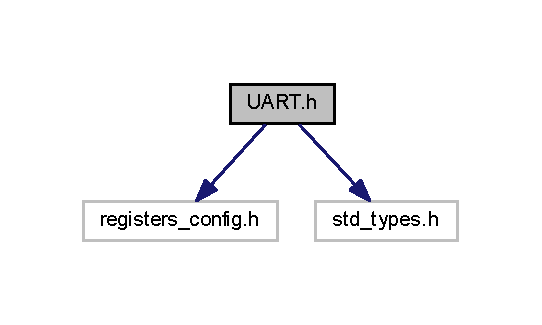
\includegraphics[width=260pt]{_u_a_r_t_8h__incl}
\end{center}
\end{figure}
This graph shows which files directly or indirectly include this file\+:\nopagebreak
\begin{figure}[H]
\begin{center}
\leavevmode
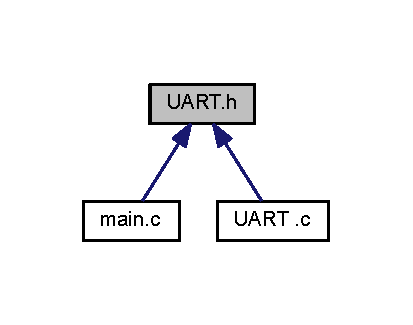
\includegraphics[width=198pt]{_u_a_r_t_8h__dep__incl}
\end{center}
\end{figure}
\subsection*{Functions}
\begin{DoxyCompactItemize}
\item 
void \hyperlink{_u_a_r_t_8h_afbfe9a19c497ec9e0586c7e6feb4897a}{uart\+\_\+init} (uint8 uart\+\_\+num)
\begin{DoxyCompactList}\small\item\em U\+A\+RT initialization \+: ~\newline
Tiva c has 8 channels for uart so the variable uart\+\_\+num is the channel number. \end{DoxyCompactList}\item 
void \hyperlink{_u_a_r_t_8h_ab0d6a19096405d3f0e1a47da77093c59}{uart\+\_\+send\+\_\+byte} (uint8 uart\+\_\+num, uint8 data)
\begin{DoxyCompactList}\small\item\em send a byte to other device \+: ~\newline
variable uart\+\_\+num for channel number specified before ~\newline
variable data for the desired data to be sent ~\newline
\end{DoxyCompactList}\item 
uint8 \hyperlink{_u_a_r_t_8h_a6672b250ddc566fa64e11ffb6d264048}{uart\+\_\+recieve\+\_\+byte} (uint8 uart\+\_\+num)
\begin{DoxyCompactList}\small\item\em receive a byte from other device \+: ~\newline
variable uart\+\_\+num is for the channel number specified before \end{DoxyCompactList}\end{DoxyCompactItemize}


\subsection{Detailed Description}
this is the library to control the serial communication between Tiva C and other microcontrollers 



\subsection{Function Documentation}
\mbox{\Hypertarget{_u_a_r_t_8h_afbfe9a19c497ec9e0586c7e6feb4897a}\label{_u_a_r_t_8h_afbfe9a19c497ec9e0586c7e6feb4897a}} 
\index{U\+A\+R\+T.\+h@{U\+A\+R\+T.\+h}!uart\+\_\+init@{uart\+\_\+init}}
\index{uart\+\_\+init@{uart\+\_\+init}!U\+A\+R\+T.\+h@{U\+A\+R\+T.\+h}}
\subsubsection{\texorpdfstring{uart\+\_\+init()}{uart\_init()}}
{\footnotesize\ttfamily void uart\+\_\+init (\begin{DoxyParamCaption}\item[{uint8}]{uart\+\_\+num }\end{DoxyParamCaption})}



U\+A\+RT initialization \+: ~\newline
Tiva c has 8 channels for uart so the variable uart\+\_\+num is the channel number. 


\begin{DoxyCode}
      \textcolor{keywordflow}{if}(uart\_num == 0)
\{
    \textcolor{keyword}{volatile} uint32 delay;
    \textcolor{comment}{/* Assumes a 16 MHz bus clock, creates 9600 baud rate */}

    \textcolor{comment}{/* Enable and provide a clock to UART module in Run mode */}
    SYSCTL\_RCGC1\_R |=(1<<uart\_num);

    \textcolor{comment}{/* allow time to finish activating */}
    delay = SYSCTL\_RCGC2\_R;

    \textcolor{comment}{/* SYSCTL\_RCGCGPIO\_R enabled by function ports\_clock\_EN() for all ports */}

    \textcolor{comment}{/*  disable UART */}
    UART0\_CTL\_R &= ~(0x00000001);

    \textcolor{comment}{/* Set the GPIO AFSEL bits to enable alternative function */}
    GPIO\_PORTA\_AFSEL\_R |= 0x03 ;

    \textcolor{comment}{/* Configure the PMCn fields in the GPIOPCTL register to assign the UART signals */}
    GPIO\_PORTA\_PCTL\_R = (GPIO\_PORTA\_PCTL\_R & 0xFFFFFF00) | (0x00000011) ;



    \textcolor{comment}{/* IBRD = int(16,000,000/(16*9600)) = int(104.1666667) */}
    UART0\_IBRD\_R = 104;

    \textcolor{comment}{/* UARTFBRD[DIVFRAC] = integer(0.166666667 * 64 + 0.5) = int(11.1666) = 11 */}
    UART0\_FBRD\_R = 11;

    \textcolor{comment}{/*  8 bit, no parity bits, one stop, disable FIFOs */}
    UART0\_LCRH\_R |= 0x00000060;

    \textcolor{comment}{/* enable UART */}
    UART0\_CTL\_R |= 0x00000301;

    \textcolor{comment}{/* The digital functions for the corresponding pin are enabled */}
    GPIO\_PORTA\_DEN\_R |= 0X03;

    \textcolor{comment}{/* disable analog on pins */}
    GPIO\_PORTA\_AMSEL\_R &= ~(0x03);
\}

\textcolor{keywordflow}{else} \textcolor{keywordflow}{if}(uart\_num == 1)
\{
    \textcolor{keyword}{volatile} uint32 delay;
    \textcolor{comment}{/* Assumes a 80 MHz bus clock, creates 9600 baud rate */}

    \textcolor{comment}{/* Enable and provide a clock to UART module in Run mode */}
    SYSCTL\_RCGC1\_R |=(1<<uart\_num);

    \textcolor{comment}{/* allow time to finish activating */}
    delay = SYSCTL\_RCGC2\_R;

    \textcolor{comment}{/* SYSCTL\_RCGCGPIO\_R enabled by function ports\_clock\_EN() for all ports */}

    \textcolor{comment}{/*  disable UART */}
    UART1\_CTL\_R &= ~(0x00000001);

    \textcolor{comment}{/* Set the GPIO AFSEL bits to enable alt funct */}
    GPIO\_PORTB\_AFSEL\_R |= 0x03 ;

    \textcolor{comment}{/* Configure the PMCn fields in the GPIOPCTL register to assign the UART signals */}
    GPIO\_PORTB\_PCTL\_R = (GPIO\_PORTA\_PCTL\_R & 0xFFFFFF00) | (0x00000011) ;



    \textcolor{comment}{/* IBRD = int(16,000,000/(16*9600)) = int(104.1666667) */}
    UART1\_IBRD\_R = 104;

    \textcolor{comment}{/* UARTFBRD[DIVFRAC] = integer(0.166666667 * 64 + 0.5) = int(11.1666) = 11 */}
    UART1\_FBRD\_R = 11;

    \textcolor{comment}{/*  8 bit, no parity bits, one stop, disable FIFOs */}
    UART1\_LCRH\_R |= 0x00000060;

    \textcolor{comment}{/* enable UART */}
    UART1\_CTL\_R |= 0x00000301;

    \textcolor{comment}{/* The digital functions for the corresponding pin are enabled */}
    GPIO\_PORTB\_DEN\_R |= 0X03;

    \textcolor{comment}{/* disable analog on pins */}
    GPIO\_PORTB\_AMSEL\_R &= ~(0x03);

\}
\textcolor{keywordflow}{else} \textcolor{keywordflow}{if}(uart\_num == 2)
\{
    \textcolor{keyword}{volatile} uint32 delay;
    \textcolor{comment}{/* Assumes a 80 MHz bus clock, creates 9600 baud rate */}

    \textcolor{comment}{/* Enable and provide a clock to UART module in Run mode */}
    SYSCTL\_RCGC1\_R |=(1<<uart\_num);

    \textcolor{comment}{/* allow time to finish activating */}
    delay = SYSCTL\_RCGC2\_R;

    \textcolor{comment}{/* SYSCTL\_RCGCGPIO\_R enabled by function ports\_clock\_EN() for all ports */}

    \textcolor{comment}{/*  disable UART */}
    UART2\_CTL\_R &= ~(0x00000001);

    \textcolor{comment}{/* Set the GPIO AFSEL bits to enable alternative function */}
    GPIO\_PORTD\_AFSEL\_R |= 0xC0 ;

    \textcolor{comment}{/* Configure the PMCn fields in the GPIOPCTL register to assign the UART signals */}
    GPIO\_PORTD\_PCTL\_R = (GPIO\_PORTA\_PCTL\_R & 0x00FFFFFF) | (0x11000000) ;

    \textcolor{comment}{/* IBRD = int(16,000,000/(16*9600)) = int(104.1666667) */}
    UART2\_IBRD\_R = 104;

    \textcolor{comment}{/* UARTFBRD[DIVFRAC] = integer(0.166666667 * 64 + 0.5) = int(11.1666) = 11 */}
    UART2\_FBRD\_R = 11;

    \textcolor{comment}{/*  8 bit, no parity bits, one stop, disable FIFOs */}
    UART2\_LCRH\_R |= 0x00000060;

    \textcolor{comment}{/* enable UART */}
    UART2\_CTL\_R |= 0x00000301;

    \textcolor{comment}{/* The digital functions for the corresponding pin are enabled */}
    GPIO\_PORTD\_DEN\_R |= 0XC0;

    \textcolor{comment}{/* disable analog on pins */}
    GPIO\_PORTD\_AMSEL\_R &= ~(0xC0);

\}

\textcolor{keywordflow}{else} \textcolor{keywordflow}{if}(uart\_num == 3)
\{
    \textcolor{keyword}{volatile} uint32 delay;
    \textcolor{comment}{/* Assumes a 80 MHz bus clock, creates 9600 baud rate */}

    \textcolor{comment}{/* Enable and provide a clock to UART module in Run mode */}
    SYSCTL\_RCGC1\_R |=(1<<uart\_num);

    \textcolor{comment}{/* allow time to finish activating */}
    delay = SYSCTL\_RCGC2\_R;

    \textcolor{comment}{/* SYSCTL\_RCGCGPIO\_R enabled by function ports\_clock\_EN() for all ports */}

    \textcolor{comment}{/*  disable UART */}
    UART3\_CTL\_R &= ~(0x00000001);

    \textcolor{comment}{/* Set the GPIO AFSEL bits to enable alternative function */}
    GPIO\_PORTC\_AFSEL\_R |= 0xC0 ;

    \textcolor{comment}{/* Configure the PMCn fields in the GPIOPCTL register to assign the UART signals */}
    GPIO\_PORTC\_PCTL\_R = (GPIO\_PORTA\_PCTL\_R & 0x00FFFFFF) | (0x11000000) ;

    \textcolor{comment}{/* IBRD = int(16,000,000/(16*9600)) = int(104.1666667) */}
    UART3\_IBRD\_R = 104;

    \textcolor{comment}{/* UARTFBRD[DIVFRAC] = integer(0.166666667 * 64 + 0.5) = int(11.1666) = 11 */}
    UART3\_FBRD\_R = 11;

    \textcolor{comment}{/*  8 bit, no parity bits, one stop, disable FIFOs */}
    UART3\_LCRH\_R |= 0x00000060;

    \textcolor{comment}{/* enable UART */}
    UART3\_CTL\_R |= 0x00000301;

    \textcolor{comment}{/* The digital functions for the corresponding pin are enabled */}
    GPIO\_PORTC\_DEN\_R |= 0XC0;

    \textcolor{comment}{/* disable analog on pins */}
    GPIO\_PORTC\_AMSEL\_R &= ~(0xC0);

\}

\textcolor{keywordflow}{else} \textcolor{keywordflow}{if}(uart\_num == 4)
\{
    \textcolor{keyword}{volatile} uint32 delay;
    \textcolor{comment}{/* Assumes a 80 MHz bus clock, creates 9600 baud rate */}

    \textcolor{comment}{/* Enable and provide a clock to UART module in Run mode */}
    SYSCTL\_RCGC1\_R |=(1<<uart\_num);

    \textcolor{comment}{/* allow time to finish activating */}
    delay = SYSCTL\_RCGC2\_R;


    \textcolor{comment}{/* SYSCTL\_RCGCGPIO\_R enabled by function ports\_clock\_EN() for all ports */}

    \textcolor{comment}{/*  disable UART */}
    UART4\_CTL\_R &= ~(0x00000001);

    \textcolor{comment}{/* Set the GPIO AFSEL bits to enable alternative function */}
    GPIO\_PORTC\_AFSEL\_R |= 0x30 ;

    \textcolor{comment}{/* Configure the PMCn fields in the GPIOPCTL register to assign the UART signals */}
    GPIO\_PORTC\_PCTL\_R = (GPIO\_PORTA\_PCTL\_R & 0xFF00FFFF) | (0x00110000) ;

    \textcolor{comment}{/* IBRD = int(16,000,000/(16*9600)) = int(104.1666667) */}
    UART4\_IBRD\_R = 104;

    \textcolor{comment}{/* UARTFBRD[DIVFRAC] = integer(0.166666667 * 64 + 0.5) = int(11.1666) = 11 */}
    UART4\_FBRD\_R = 11;

    \textcolor{comment}{/*  8 bit, no parity bits, one stop, disable FIFOs */}
    UART4\_LCRH\_R |= 0x00000060;

    \textcolor{comment}{/* enable UART */}
    UART4\_CTL\_R |= 0x00000301;

    \textcolor{comment}{/* The digital functions for the corresponding pin are enabled */}
    GPIO\_PORTC\_DEN\_R |= 0X30;

    \textcolor{comment}{/* disable analog on pins */}
    GPIO\_PORTC\_AMSEL\_R &= ~(0x30);

\}

\textcolor{keywordflow}{else} \textcolor{keywordflow}{if}(uart\_num == 5)
\{
    \textcolor{keyword}{volatile} uint32 delay;
    \textcolor{comment}{/* Assumes a 80 MHz bus clock, creates 9600 baud rate */}

    \textcolor{comment}{/* Enable and provide a clock to UART module in Run mode */}
    SYSCTL\_RCGC1\_R |=(1<<uart\_num);

    \textcolor{comment}{/* allow time to finish activating */}
    delay = SYSCTL\_RCGC2\_R;


    \textcolor{comment}{/* SYSCTL\_RCGCGPIO\_R enabled by function ports\_clock\_EN() for all ports */}

    \textcolor{comment}{/*  disable UART */}
    UART5\_CTL\_R &= ~(0x00000001);

    \textcolor{comment}{/* Set the GPIO AFSEL bits to enable alternative function */}
    GPIO\_PORTE\_AFSEL\_R |= 0x03 ;

    \textcolor{comment}{/* Configure the PMCn fields in the GPIOPCTL register to assign the UART signals */}
    GPIO\_PORTE\_PCTL\_R = (GPIO\_PORTA\_PCTL\_R & 0xFFFFFF00) | (0x00000011) ;

    \textcolor{comment}{/* IBRD = int(16,000,000/(16*9600)) = int(104.1666667) */}
    UART5\_IBRD\_R = 104;

    \textcolor{comment}{/* UARTFBRD[DIVFRAC] = integer(0.166666667 * 64 + 0.5) = int(11.1666) = 11 */}
    UART5\_FBRD\_R = 11;

    \textcolor{comment}{/*  8 bit, no parity bits, one stop, disable FIFOs */}
    UART5\_LCRH\_R |= 0x00000060;

    \textcolor{comment}{/* enable UART */}
    UART5\_CTL\_R |= 0x00000301;

    \textcolor{comment}{/* The digital functions for the corresponding pin are enabled */}
    GPIO\_PORTE\_DEN\_R |= 0X03;

    \textcolor{comment}{/* disable analog on pins */}
    GPIO\_PORTE\_AMSEL\_R &= ~(0x03);

\}

\textcolor{keywordflow}{else} \textcolor{keywordflow}{if}(uart\_num == 6)
\{
    \textcolor{keyword}{volatile} uint32 delay;
    \textcolor{comment}{/* Assumes a 80 MHz bus clock, creates 9600 baud rate */}

    \textcolor{comment}{/* Enable and provide a clock to UART module in Run mode */}
    SYSCTL\_RCGC1\_R |=(1<<uart\_num);

    \textcolor{comment}{/* allow time to finish activating */}
    delay = SYSCTL\_RCGC2\_R;

    \textcolor{comment}{/* SYSCTL\_RCGCGPIO\_R enabled by function ports\_clock\_EN() for all ports */}

    \textcolor{comment}{/*  disable UART */}
    UART6\_CTL\_R &= ~(0x00000001);

    \textcolor{comment}{/* Set the GPIO AFSEL bits to enable alternative function */}
    GPIO\_PORTD\_AFSEL\_R |= 0x30 ;

    \textcolor{comment}{/* Configure the PMCn fields in the GPIOPCTL register to assign the UART signals */}
    GPIO\_PORTD\_PCTL\_R = (GPIO\_PORTA\_PCTL\_R & 0xFF00FFFF) | (0x00110000) ;

    \textcolor{comment}{/* IBRD = int(16,000,000/(16*9600)) = int(104.1666667) */}
    UART6\_IBRD\_R = 104;

    \textcolor{comment}{/* UARTFBRD[DIVFRAC] = integer(0.166666667 * 64 + 0.5) = int(11.1666) = 11 */}
    UART6\_FBRD\_R = 11;

    \textcolor{comment}{/*  8 bit, no parity bits, one stop, disable FIFOs */}
    UART6\_LCRH\_R |= 0x00000060;

    \textcolor{comment}{/* enable UART */}
    UART6\_CTL\_R |= 0x00000301;

    \textcolor{comment}{/* The digital functions for the corresponding pin are enabled */}
    GPIO\_PORTD\_DEN\_R |= 0X30;

    \textcolor{comment}{/* disable analog on pins */}
    GPIO\_PORTD\_AMSEL\_R &= ~(0x30);

\}

\textcolor{keywordflow}{else} \textcolor{keywordflow}{if}(uart\_num == 7)
\{
    \textcolor{keyword}{volatile} uint32 delay;
    \textcolor{comment}{/* Assumes a 80 MHz bus clock, creates 9600 baud rate */}

    \textcolor{comment}{/* Enable and provide a clock to UART module in Run mode */}
    SYSCTL\_RCGC1\_R |=(1<<uart\_num);

    \textcolor{comment}{/* allow time to finish activating */}
    delay = SYSCTL\_RCGC2\_R;

    \textcolor{comment}{/* SYSCTL\_RCGCGPIO\_R enabled by function ports\_clock\_EN() for all ports */}

    \textcolor{comment}{/*  disable UART */}
    UART7\_CTL\_R &= ~(0x00000001);

    \textcolor{comment}{/* Set the GPIO AFSEL bits to enable alternative function */}
    GPIO\_PORTE\_AFSEL\_R |= 0x03 ;

    \textcolor{comment}{/* Configure the PMCn fields in the GPIOPCTL register to assign the UART signals */}
    GPIO\_PORTE\_PCTL\_R = (GPIO\_PORTA\_PCTL\_R & 0xFFFFFF00) | (0x00000011) ;

    \textcolor{comment}{/* IBRD = int(16,000,000/(16*9600)) = int(104.1666667) */}
    UART7\_IBRD\_R = 104;

    \textcolor{comment}{/* UARTFBRD[DIVFRAC] = integer(0.166666667 * 64 + 0.5) = int(11.1666) = 11 */}
    UART7\_FBRD\_R = 11;

    \textcolor{comment}{/*  8 bit, no parity bits, one stop, disable FIFOs */}
    UART7\_LCRH\_R |= 0x00000060;

    \textcolor{comment}{/* enable UART */}
    UART7\_CTL\_R |= 0x00000301;

    \textcolor{comment}{/* The digital functions for the corresponding pin are enabled */}
    GPIO\_PORTE\_DEN\_R |= 0X03;

    \textcolor{comment}{/* disable analog on pins */}
    GPIO\_PORTE\_AMSEL\_R &= ~(0x03);

\}


\}
\end{DoxyCode}
 \mbox{\Hypertarget{_u_a_r_t_8h_a6672b250ddc566fa64e11ffb6d264048}\label{_u_a_r_t_8h_a6672b250ddc566fa64e11ffb6d264048}} 
\index{U\+A\+R\+T.\+h@{U\+A\+R\+T.\+h}!uart\+\_\+recieve\+\_\+byte@{uart\+\_\+recieve\+\_\+byte}}
\index{uart\+\_\+recieve\+\_\+byte@{uart\+\_\+recieve\+\_\+byte}!U\+A\+R\+T.\+h@{U\+A\+R\+T.\+h}}
\subsubsection{\texorpdfstring{uart\+\_\+recieve\+\_\+byte()}{uart\_recieve\_byte()}}
{\footnotesize\ttfamily uint8 uart\+\_\+recieve\+\_\+byte (\begin{DoxyParamCaption}\item[{uint8}]{uart\+\_\+num }\end{DoxyParamCaption})}



receive a byte from other device \+: ~\newline
variable uart\+\_\+num is for the channel number specified before 


\begin{DoxyCode}
 \{
    \textcolor{comment}{/* function to recieve byte takes one input (uart number)}
\textcolor{comment}{     * return recieved byte  */}

    \textcolor{keywordflow}{if}(uart\_num == 0)
    \{
        \textcolor{comment}{/* Wait for new input ,wait until RXFE is 0 */}
        \textcolor{keywordflow}{while}((UART0\_FR\_R & 0x0010) != 0);
        \textcolor{keywordflow}{return} ((uint8)(UART0\_DR\_R & 0xFF)) ;

    \}

    \textcolor{keywordflow}{else} \textcolor{keywordflow}{if}(uart\_num == 1)
    \{
        \textcolor{comment}{/* Wait for new input ,wait until RXFE is 0 */}
        \textcolor{keywordflow}{while}((UART1\_FR\_R & 0x0010) != 0)\{\}
        \textcolor{keywordflow}{return} ((uint8)(UART1\_DR\_R & 0xFF)) ;
    \}

    \textcolor{keywordflow}{else} \textcolor{keywordflow}{if}(uart\_num == 2)
    \{
        \textcolor{comment}{/* Wait for new input ,wait until RXFE is 0 */}
        \textcolor{keywordflow}{while}((UART2\_FR\_R & 0x0010) != 0);
        \textcolor{keywordflow}{return} ((uint8)(UART2\_DR\_R & 0xFF)) ;
    \}

    \textcolor{keywordflow}{else} \textcolor{keywordflow}{if}(uart\_num == 3)
    \{
        \textcolor{comment}{/* Wait for new input ,wait until RXFE is 0 */}
        \textcolor{keywordflow}{while}((UART3\_FR\_R & 0x0010) != 0);
        \textcolor{keywordflow}{return} ((uint8)(UART3\_DR\_R & 0xFF)) ;
    \}

    \textcolor{keywordflow}{else} \textcolor{keywordflow}{if}(uart\_num == 4)
    \{
        \textcolor{comment}{/* Wait for new input ,wait until RXFE is 0 */}
        \textcolor{keywordflow}{while}((UART4\_FR\_R & 0x0010) != 0);
        \textcolor{keywordflow}{return} ((uint8)(UART4\_DR\_R & 0xFF)) ;
    \}

    \textcolor{keywordflow}{else} \textcolor{keywordflow}{if}(uart\_num == 5)
    \{
        \textcolor{comment}{/* Wait for new input ,wait until RXFE is 0 */}
        \textcolor{keywordflow}{while}((UART5\_FR\_R & 0x0010) != 0);
        \textcolor{keywordflow}{return} ((uint8)(UART5\_DR\_R & 0xFF)) ;
    \}

    \textcolor{keywordflow}{else} \textcolor{keywordflow}{if}(uart\_num == 6)
    \{
        \textcolor{comment}{/* Wait for new input ,wait until RXFE is 0 */}
        \textcolor{keywordflow}{while}((UART6\_FR\_R & 0x0010) != 0);
        \textcolor{keywordflow}{return} ((uint8)(UART6\_DR\_R & 0xFF)) ;
    \}

    \textcolor{keywordflow}{else} \textcolor{keywordflow}{if}(uart\_num == 7)
    \{
        \textcolor{comment}{/* Wait for new input ,wait until RXFE is 0 */}
        \textcolor{keywordflow}{while}((UART7\_FR\_R & 0x0010) != 0);
        \textcolor{keywordflow}{return} ((uint8)(UART7\_DR\_R & 0xFF)) ;
    \}


\}
\end{DoxyCode}
 \mbox{\Hypertarget{_u_a_r_t_8h_ab0d6a19096405d3f0e1a47da77093c59}\label{_u_a_r_t_8h_ab0d6a19096405d3f0e1a47da77093c59}} 
\index{U\+A\+R\+T.\+h@{U\+A\+R\+T.\+h}!uart\+\_\+send\+\_\+byte@{uart\+\_\+send\+\_\+byte}}
\index{uart\+\_\+send\+\_\+byte@{uart\+\_\+send\+\_\+byte}!U\+A\+R\+T.\+h@{U\+A\+R\+T.\+h}}
\subsubsection{\texorpdfstring{uart\+\_\+send\+\_\+byte()}{uart\_send\_byte()}}
{\footnotesize\ttfamily void uart\+\_\+send\+\_\+byte (\begin{DoxyParamCaption}\item[{uint8}]{uart\+\_\+num,  }\item[{uint8}]{data }\end{DoxyParamCaption})}



send a byte to other device \+: ~\newline
variable uart\+\_\+num for channel number specified before ~\newline
variable data for the desired data to be sent ~\newline



\begin{DoxyCode}
  \{
    \textcolor{comment}{/* void function to send byte takes data and uart number  */}
    \textcolor{keywordflow}{if}(uart\_num == 0)
    \{
        \textcolor{comment}{/* Wait for buffer to be not full ,TXFF to be clear */}
        \textcolor{keywordflow}{while}((UART0\_FR\_R & 0x0020) != 0)\{\}
        UART0\_DR\_R = data ;

    \}

    \textcolor{keywordflow}{else} \textcolor{keywordflow}{if}(uart\_num == 1)
    \{
        \textcolor{comment}{/* Wait for buffer to be not full ,TXFF to be clear */}
        \textcolor{keywordflow}{while}((UART1\_FR\_R & 0x0020) != 0)\{\}
        UART1\_DR\_R = data ;
    \}

    \textcolor{keywordflow}{else} \textcolor{keywordflow}{if}(uart\_num == 2)
    \{
        \textcolor{comment}{/* Wait for buffer to be not full ,TXFF to be clear */}
        \textcolor{keywordflow}{while}((UART2\_FR\_R & 0x0020) != 0);
        UART2\_DR\_R = data ;
    \}

    \textcolor{keywordflow}{else} \textcolor{keywordflow}{if}(uart\_num == 3)
    \{
        \textcolor{comment}{/* Wait for buffer to be not full ,TXFF to be clear */}
        \textcolor{keywordflow}{while}((UART3\_FR\_R & 0x0020) != 0);
        UART3\_DR\_R = data ;

    \}

    \textcolor{keywordflow}{else} \textcolor{keywordflow}{if}(uart\_num == 4)
    \{
        \textcolor{comment}{/* Wait for buffer to be not full ,TXFF to be clear */}
        \textcolor{keywordflow}{while}((UART4\_FR\_R & 0x0020) != 0);
        UART4\_DR\_R = data ;
    \}

    \textcolor{keywordflow}{else} \textcolor{keywordflow}{if}(uart\_num == 5)
    \{
        \textcolor{comment}{/* Wait for buffer to be not full ,TXFF to be clear */}
        \textcolor{keywordflow}{while}((UART5\_FR\_R & 0x0020) != 0);
        UART5\_DR\_R = data ;
    \}

    \textcolor{keywordflow}{else} \textcolor{keywordflow}{if}(uart\_num == 6)
    \{
        \textcolor{comment}{/* Wait for buffer to be not full ,TXFF to be clear */}
        \textcolor{keywordflow}{while}((UART6\_FR\_R & 0x0020) != 0);
        UART6\_DR\_R = data ;
    \}

    \textcolor{keywordflow}{else} \textcolor{keywordflow}{if}(uart\_num == 7)
    \{
        \textcolor{comment}{/* Wait for buffer to be not full ,TXFF to be clear */}
        \textcolor{keywordflow}{while}((UART7\_FR\_R & 0x0020) != 0);
        UART7\_DR\_R = data ;
    \}
\}
\end{DoxyCode}
 
%--- End generated contents ---

% Index
\backmatter
\newpage
\phantomsection
\clearemptydoublepage
\addcontentsline{toc}{chapter}{Index}
\printindex

\end{document}
